\section{Introduction} % Sections are added in order to organize your presentation into discrete blocks, all sections and subsections are automatically output to the table of contents as an overview of the talk but NOT output in the presentation as separate slides

\begin{frame}{Preliminaries}
	\begin{columns}[T] % The "T" option aligns the columns' content at the top
		% Left column
		\begin{column}{0.5\textwidth} % Adjust the width of the column as you like
			\begin{itemize}
				\item C++ based implementation using \texttt{OpenMP} and \texttt{Eigen3}.
				\item \texttt{main.cpp} as center of application
				\item \texttt{particle.c/hpp} Holds Particle3D class with relevant members
				\item \texttt{data.c/hpp} reads in file
				\item \texttt{histogram.c/hpp} and \texttt{shell.c/hpp} handle histogram creation and binning
				\item \texttt{system.c/hpp} Relevant and global constants and factors
				\item \texttt{treecode.c/hpp} Multipole expansion related class and methods
			\end{itemize}
		\end{column}

		% Right column
		\begin{column}{0.5\textwidth} % Adjust the width of the column as you like
			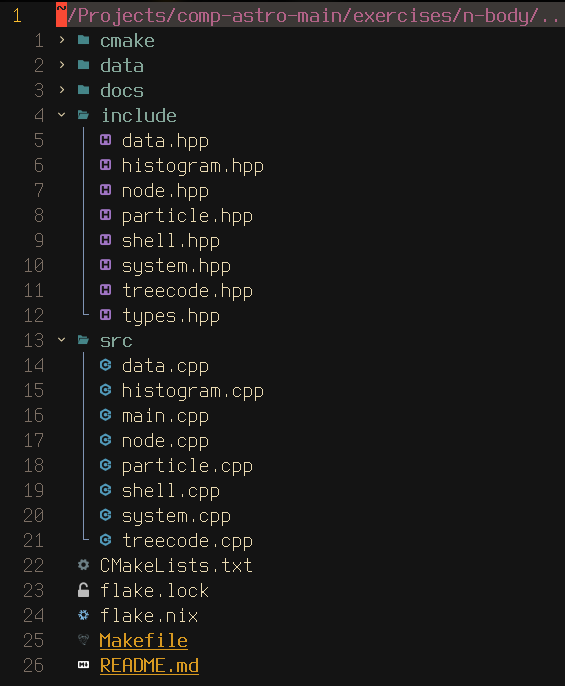
\includegraphics[width=\textwidth]{figures/source-tree}
		\end{column}
	\end{columns}
\end{frame}

\begin{frame}{Units and Dimension}
	From assumption $G=1$ follows: \\
	Dimensionless Quantities:
	\begin{equation}
		\vb{r}^{\prime}=\frac{\vb{r}}{R_0}, \quad m^{\prime}=\frac{m}{M_0}, \quad t^{\prime}=\frac{t}{T_0}
	\end{equation}
	Derived quantities for consistency:
	\begin{equation}
		\begin{aligned}
			\vb{v}^{\prime} = \frac{\vb{v}}{V_0} = \vb{v} \frac{T_0}{R_0}, \quad \vb{a}^{\prime} = \frac{\vb{a}}{A_0} = \vb{a} \frac{T_0^2}{R_0}
		\end{aligned}
	\end{equation}
	Repercussions for setting $G = 1$
	\begin{equation}
		\begin{aligned}
			\vb{a}_i                      & =-G \sum_{j\neq i} m_j \frac{\vb{r}_i-\vb{r}_j}{\left|\vb{r}_i-\vb{r}_j\right|^3} \\
			\Rightarrow \vb{a}_i^{\prime} & =\underbrace{\left\{\frac{G M_0
					T_0^2}{R_0^3}\right\}}_{G^{\prime}} \sum_{j\neq i} m_j^\prime
			\frac{\vb{r}_i^\prime-\vb{r}^\prime_j}{\left|\vb{r}^\prime_i-\vb{r}^\prime_j\right|^3}
		\end{aligned}
	\end{equation}
\end{frame}

\begin{frame}{Defining Units}
	Time scaling factor $T_0$:
	\begin{equation}
		\frac{G M_0 T_0^2}{R_0^3}=1 \quad \Rightarrow \quad T_0=\left(\frac{R_0^3}{G M_0}\right)^{1 / 2}
	\end{equation}\bigskip

	Where:
	\begin{itemize}
		\item $T_0 \simeq 14.91 Myr$
		\item $M_0 =  1 M_\odot$.
		\item $R_0 =  1 pc$.
		\item $V_0 \simeq 0.065 \frac{km}{s} \simeq 0.067 \frac{pc}{Myr}$
		\item $A_0 \simeq 0.004 \frac{pc}{Myr^2}$
	\end{itemize}
	% Data from file assumed as $M_\odot$, $pc$ and $\frac{km}{s}$
\end{frame}
